\chapter{پیشینه تحقیق}
\usetikzlibrary{shapes.geometric, arrows}

\tikzstyle{startstop} = [rectangle, rounded corners, minimum width=3cm, minimum height=1cm,text centered, draw=black, fill=red!30]
\tikzstyle{process} = [rectangle, minimum width=3cm, minimum height=1cm, text centered, draw=black, fill=orange!30]
\tikzstyle{arrow} = [thick,->,>=stealth]


	
	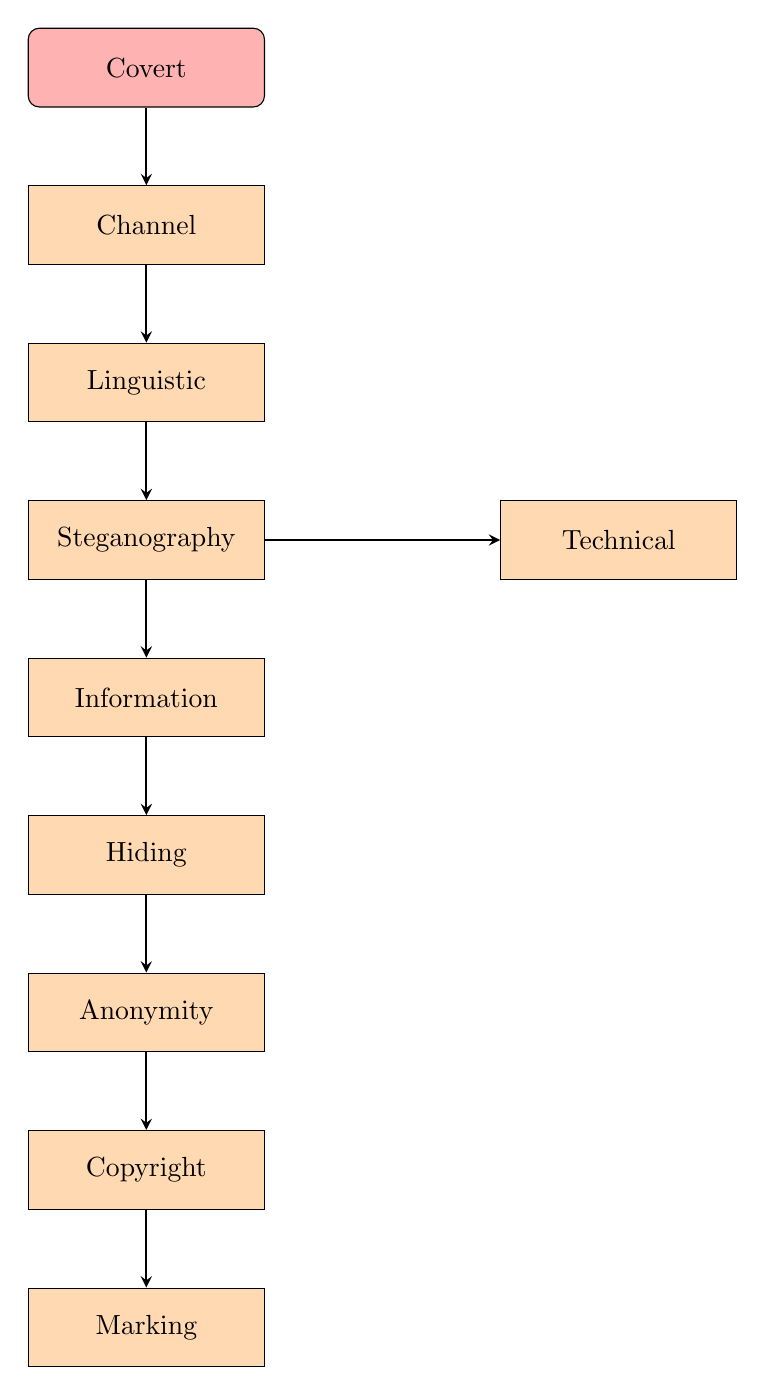
\begin{tikzpicture}[node distance=2cm]
		
		\node (Covert) [startstop] {Covert};
		\node (Channel) [process, below of=Covert] {Channel};
		\node (Linguistic) [process, below of=Channel] {Linguistic};
		\node (Steganography) [process, below of=Linguistic] {Steganography};
		\node (Technical) [process, right of=Steganography, xshift=4cm] {Technical};
		\node (Information) [process, below of=Steganography] {Information};
		\node (Hiding) [process, below of=Information] {Hiding};
		\node (Anonymity) [process, below of=Hiding] {Anonymity};
		\node (Copyright) [process, below of=Anonymity] {Copyright};
		\node (Marking) [process, below of=Copyright] {Marking};
		
		\draw [arrow] (Covert) -- (Channel);
		\draw [arrow] (Channel) -- (Linguistic);
		\draw [arrow] (Linguistic) -- (Steganography);
		\draw [arrow] (Steganography) -- (Information);
		\draw [arrow] (Information) -- (Hiding);
		\draw [arrow] (Hiding) -- (Anonymity);
		\draw [arrow] (Anonymity) -- (Copyright);
		\draw [arrow] (Copyright) -- (Marking);
		\draw [arrow] (Steganography) -- (Technical);
		
	\end{tikzpicture}